\documentclass{nsfproposal}
\usepackage{amsmath, amsthm, epsfig}
\usepackage{subfigure}
\usepackage{url}
\usepackage{wrapfig}
\usepackage{color}
\usepackage{graphicx}
\usepackage{array}
\usepackage{setspace}
\usepackage[font={small,sf},labelfont={small,sf,bf}]{caption}



\makeatletter
\setlength\itemsep{1\p@}
\setlength\leftmargini{2.em}
\setlength\belowcaptionskip{.25ex \@plus -.8ex \@minus -.2ex}
\setlength\abovecaptionskip{-2pt}


\renewcommand\section{\@startsection {section}{1}{\z@}%
                                   {-1.5ex \@plus -2ex \@minus -.2ex}%
                                   {.25ex \@plus.2ex}%
                                   {\normalfont\Large\bfseries}}
\renewcommand\subsection{\@startsection{subsection}{2}{\z@}%
                                   {-1.2ex \@plus -2ex \@minus -.2ex}%
                                   {.25ex \@plus.2ex}%
	                           {\normalfont\large\bfseries}}
\renewcommand\subsubsection{\@startsection{subsubsection}{3}{\z@}%
                                     {-.55ex\@plus -.2ex \@minus -.2ex}%
                                     {.2ex \@plus .2ex}%
                                     {\normalfont\large\bfseries}}


\abovedisplayskip=5pt plus 3pt minus 6pt
\abovedisplayshortskip=0pt plus 3pt
\belowdisplayskip=5pt plus 3pt minus 6pt
\belowdisplayshortskip=3pt plus 3pt minus 4pt

\floatsep 6pt plus 2pt minus 2pt
\textfloatsep 6pt plus 2pt minus 4pt
\intextsep 6pt plus 2pt minus 2pt
\dblfloatsep 4pt plus 2pt minus 2pt
\dbltextfloatsep 4pt plus 2pt minus 4pt
\@fptop 0pt plus 1fil \@fpsep 6pt plus 2fil \@fpbot 0pt plus 1fil
\@dblfptop 0pt plus 1fil \@dblfpsep 6pt plus 2fil \@dblfpbot 0pt plus 1fil



\makeatother


% NSF proposal generation template style file.
% based on latex stylefiles  written by Stefan Llewellyn Smith and
% Sarah Gille, with contributions from Tboult and  others.
% Further customized by David Cox and Walter Scheirer

\newcommand{\degrees}{$\!\!$\char23$\!$}
\DeclareFontFamily{OT1}{psyr}{}
\DeclareFontShape{OT1}{psyr}{m}{n}{<-> psyr}{}
\def\times{{\fontfamily{psyr}\selectfont\char180}}


\renewcommand{\refname}{\centerline{References cited}}

% this handles hanging indents for publications
\def\rrr#1\\{\par
\medskip\hbox{\vbox{\parindent=2em\hsize=6.12in
\hangindent=4em\hangafter=1#1}}}

\def\baselinestretch{1}
\newcommand{\argmin}{\operatornamewithlimits{argmin}}
\def\real{\mathbb{R}}
\def\expeted{\mathbb{E}}
\long\def\comment#1{}
\theoremstyle{definition}
\newtheorem{mydef}{Definition}
\newtheorem{myaim}{Objective}




\begin{document}

% -------------------------------------------
% PROJECT SUMMARY
% -------------------------------------------


\begin{center}
{\Large{\bf Project Summary}}\\
{\bf \large The Title Goes Here
} \\
IIS: Robust Intelligence: Medium
\\*[3mm]

David Cox (Harvard University) and XXX (XXX)

\end{center}


A summary of the proposal goes here, takes two-third of page.

\vspace{1ex}
\noindent
{\bf Intellectual Merit:} xxxTODO The proposed work will [do something really intellectually meritorious].  A paragraph or two.

\vspace{1ex}
\noindent
{\bf Broader Impacts:} xxxTODO Discussion of broader impact; educational outreach, impact on other outside fields, social/commercial/etc. impacts.  A paragraph or two.


\renewcommand{\thepage} {A--\arabic{page}}

\newpage


\pagenumbering{arabic}
\renewcommand{\thepage} {C--\arabic{page}}

\newpage

% -------------------------------------------
% Project Description
%
%  15 pages
%  + *additional 2* for collaboration plan for
%    medium & large collaborative proposals
%
% -------------------------------------------

\section{Overview of Project Objectives}

%  1-2 PAGES
% Intro goes here
While large strides have been made towards ...

The elements of our interdisciplinary project are summarized in Fig.~\ref{fig:overview}, with three main areas of contribution ...

\begin{figure}[!b]
\centering
\includegraphics [scale=0.38]{figures/overview.pdf}
\vspace{2mm}
\caption{Overview of the Project: xxxx}
\label{fig:overview}
\end{figure}


\vspace{.5ex}
\begin{myaim}
{\bf Do something transformative}: a brief description of the transformative thing in a few sentences.
\end{myaim}
\vspace*{-1.1ex}
\hangindent=10pt \ This task represents the core of our project: lorem ipsum and so on...

\vspace{.5ex}
\begin{myaim}
{\bf Demonstrate Something else}: develop new algorithms that are super awesome
\end{myaim}
\vspace*{-1.1ex}
\hangindent=10pt \ Some more explanatory text

\vspace{.5ex}
\begin{myaim}
{\bf And so on so forth}: Develop new algorithms that do something.
\end{myaim}
\vspace*{-1.1ex}
\hangindent=10pt \ More explanatory paragraphs

\vspace{.5ex}
\begin{myaim}
{\bf Interdisciplinary Impact}: Through educational and research-oriented outreach, bring together xxxx....
\end{myaim}
\vspace*{-1.1ex}
\hangindent=10pt \ Our team's interdisciplinary nature provides strength in both core vision science and computer vision...

\section{Background}

% ~ 1 PAGE

Good grant proposals have some background...
\label{sec:background}

% ---------------------------------------------
% Describe objectives
% ---------------------------------------------

%\input{asubsection.tex}
%\label{sec:asubsection}


% ---------------------------------------------
% Required Elements
% ---------------------------------------------

\section{Education and Outreach }
\label{sec:edu}

% 0.5 PAGE
The educational and outreach activities associated with this project will be two-fold.
First, to engage with the broader academic community, we propose to ...

A paragraph or two about this.

Second, to engage with the public, we will ...

A paragraph or two about that





\section{Project Timeline}
\label{sec:man}

% 1 paragraph or so + (optional) figure

\begin{figure*}[t]
\centering
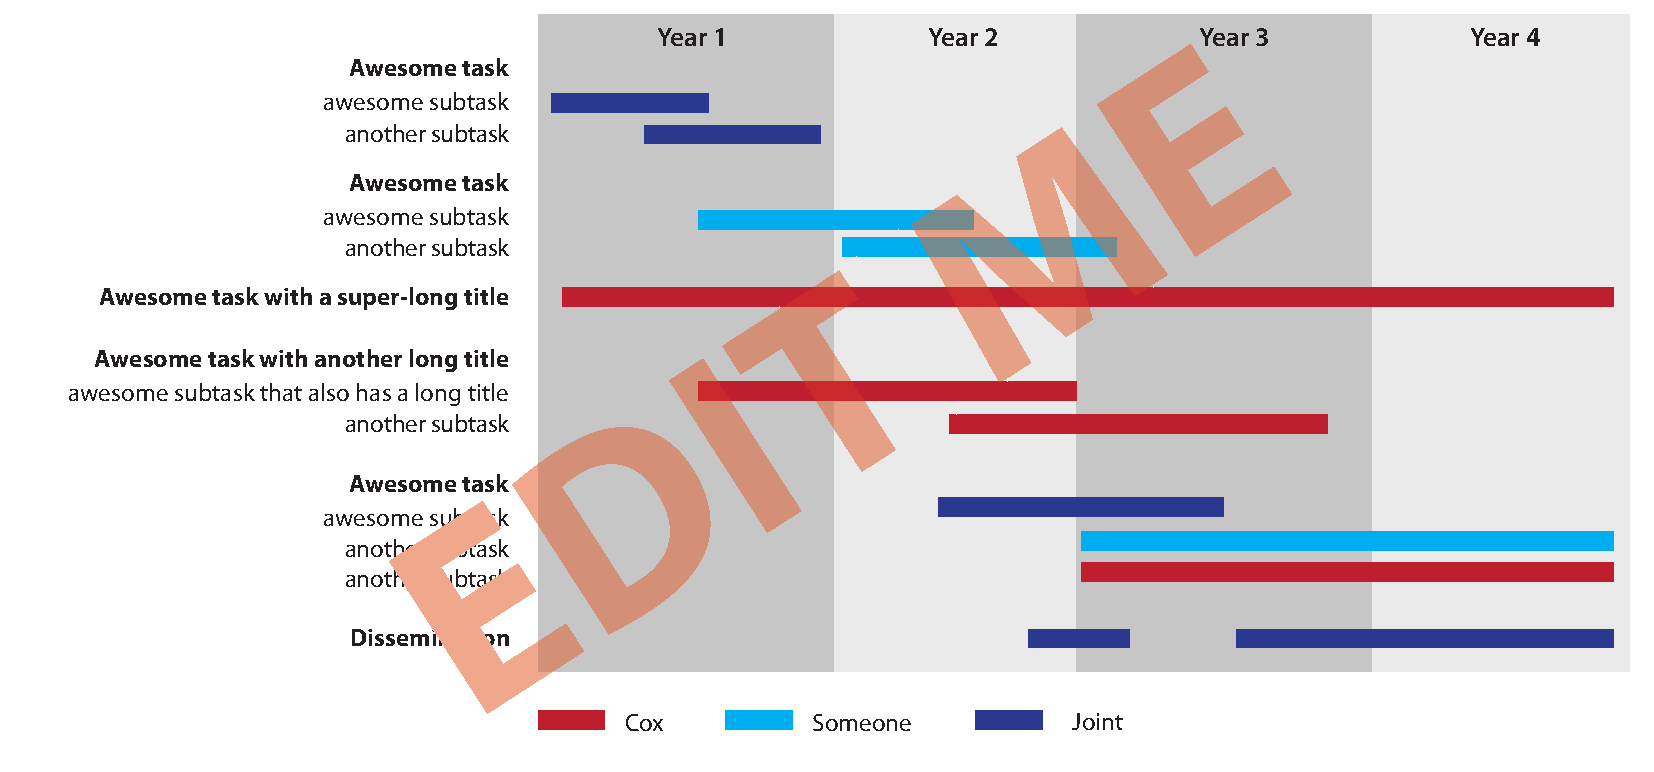
\includegraphics [width=0.97\linewidth]{figures/timeline.pdf}
\label{fig:timeline}
\end{figure*}

The proposed effort will be staged according to the timeline shown below, with
tightly integrated periods of joint effort between both groups throughout the project timeline.
Dissemination of sharable materials will occur as they become available, with a focused period
of preparation of materials for dissemination in the third and fourth years.



\section{Evaluation Plan}
\label{sec:eval}

% 0.5 PAGE
Continual evaluation of the effectiveness of our efforts will be essential to project success.
First, where standard benchmark datasets exist, we will test the algorithms resulting from the present project using these sets.
... xxxx


\section{Results from Recent Prior NSF Support}
\label{sec:prior}

% try to keep it to 1-2 pages, use lots of citations as needed but keep the text short
\noindent

% Cox results from previous NSF
In his role as PI on NSF EAGER Award IOS 0947777: ``A Novel Rodent Model for the Neurophysiology of Visual Object Recognition'' (09/09-09/11), {\bf Prof. Cox} developed infrastructure and performed experiments establishing the laboratory rat as a powerful new model system for studying the neurophysiological underpinnings of high-level visual recognition. This work resulted in one journal publication \cite{zoccolan:frontiers_2010}, with two more publications currently in preparation, and resulted in open source software and hardware being made available for novel experimental apparatus. This project also engaged two REU students, both of whom have gone on to pursue STEM careers.

As Co-PI on NSF Award IIS 0963668: ``Collaborative Research: Unlocking Biologically-Inspired Computer Vision: A High-Throughput Approach'' (09/10-09/13), {\bf Prof. Cox} has made significant contributions to advancing understanding of biologically-inspired machine vision algorithms, as well as making contributions to general high-performance computing techniques required for running them efficiently at scale.
While this project is still in ongoing, it has already resulted in eight peer-reviewed publications \cite{vig:eccv_2012, bergstra:inpar_2012, vig:icip_2012, pinto:fg_2011, pinto:bionetics_2010, pinto:gcg2, pinto:cvpr_ws_2011, pinto:imavis_2012, chiachia:bmvc_2012}.  To date, this project has engaged one REU student, and has supported the organization of a workshop at the IEEE CVPR 2011 conference designed to bring together the neuroscience and computer vision community.


% Scheirer results from previous
In his role as PI on NSF STTR \#0750485 (3/1/2007-2/28/2011) on Improving Privacy and Security of Biometrics Systems, \textbf{Dr. Scheirer} made significant advancements in biometric-based technology for security and privacy, leading to the only PayPal approved application using fingerprint technology for financial transactions. This project has engaged more than a dozen undergraduates at the University of Colorado, Colorado Springs (several as REU students), five UCCS graduate students, and two high school interns (both RAHSS students). It has led to several publications~\cite{biotoken-07, cracking, biocrypt, bipartite-icb-09, BKI-Wifs, scheirer_2012_bki}.

Under NSF Award IIS-1136370 (4/15/2011 - 3/31/2012) ``Group Travel Grant for the Doctoral Consortium at the IEEE Conference on Computer Vision and Pattern Recognition" \textbf{Dr. Scheirer} as PI organized the doctoral consortium event at CVPR 2011, the premier conference in the area of computer vision.

% Other results from previous
%\input{other_previous.tex}


% ---------------------------------------------
% Collaboration Plan
% ---------------------------------------------

\newpage
\pagenumbering{arabic}
\renewcommand{\thepage} {D--\arabic{page}}


\section{Collaboration Plan}
\label{sec:collab}

\subsection{Advantage of the collaboration}

% Collaboration Plans for Medium and Large Proposals - Since the success of collaborative research efforts are known to depend on thoughtful coordination mechanisms that regularly bring together the various participants of the project, all Medium proposals that include more than one investigator and all Large proposals must include a Collaboration Plan. While the length of the Project Description for Small and Medium proposals is limited to 15 pages and for Large proposals to 20 pages, for Medium and Large proposals up to 2 additional pages are allowed for Collaboration Plans. Collaboration Plans should be included at the end of the Project Description in a section entitled "Collaboration Plan". The length of and degree of detail provided in the Collaboration Plan should be commensurate with the complexity of the proposed project. Where appropriate, the Collaboration Plan might include: 1) the specific roles of the project participants in all organizations involved; 2) information on how the project will be managed across all the investigators, institutions, and/or disciplines; 3) identification of the specific coordination mechanisms that will enable cross-investigator, cross-institution, and/or cross-discipline scientific integration (e.g., yearly workshops, graduate student exchange, project meetings at conferences, use of the grid for videoconferences, software repositories, etc.), and 4) specific references to the budget line items that support collaboration and coordination mechanisms. If a Large proposal, or a Medium proposal with more than one investigator, does not include a Collaboration Plan of up to 2 pages, that proposal will be returned without review.

% tl;dr - 2 pages on how we'll play nice together

We have proposed here a program of work that brings together two laboratories from different departments and disciplines, with highly complementary expertise, to tackle a novel point of intersection and interaction between the fields of xxxx.
The proposed work requires a team with skills in computer science, engineering, neuroscience, and psychology --- a diverse skillset that the current team is uniquely well-positioned to provide.

Specifically, the skills of the key personnel currently on the team are:

David D. Cox, Ph.D., (co-Principal Investigator) is an Assistant Professor of Molecular and Cellular Biology at Harvard University, and a member of the Harvard Center for Brain Science. He has an extensive background in both computer science and neuroscience. His laboratory's efforts are organized along two concerted fronts: reverse engineering simple biological visual systems (using rodents as a model system), and using resulting knowledge to forward engineer biologically-inspired artificial systems using high performance computing tools.

....

Walter J. Scheirer, Ph.D. (Senior Personnel) is a senior postdoctoral fellow in Prof. Cox's Laboratory.  He is also an Assistant Professor Adjoint at the University of Colorado, Colorado Springs. Previously, he was the director of research \& development at Securics, Inc., an early stage company producing innovative computer vision-based solutions. Dr. Scheirer has extensive experience in the areas of computer vision and human biometrics, with an emphasis on advanced learning techniques. His overarching research interest is the fundamental problem of recognition, including the representations and algorithms supporting solutions to it.


\subsection{Roles of the team members}

The proposed work will be carried out by a highly interdisciplinary team of researchers.  Specific responsibilities within the group are described below.

The Cox Lab team will:

\begin{itemize}
\item do something
\item do something else
\end{itemize}

The xxxx team will:

\begin{itemize}
\item spearhead efforts to do something
\item do something else
\end{itemize}


\subsection{Managerial arrangements}

The co-PIs have extensively discussed and agreed upon the proposed research directions, and [xxxx will do awesome collab stuff together]
The two labs will perform the proposed work in a highly interactive manner, with team members interacting on a day-to-day basis, but with a minimum of bi-weekly meetings attended by both groups.
Both PIs anticipate being coauthors on all papers resulting from the proposed work.
The specific budget provided by each lab for this proposal indicates how project funds will be divided and spent in each group.
Prof. Cox [xxx TODO] will take the lead in administrative interaction with the NSF.
Progress reports will be prepared jointly.



\newpage


% ---------------------------------------------
% References
% ---------------------------------------------

\pagenumbering{arabic}
\renewcommand{\thepage} {E--\arabic{page}}

% include bib files, comma separated WITHOUT spaces
\bibliography{coxlab_publications,refs}

\bibliographystyle{plain}

\end{document}
